%%% Analyse for optimering af Current-sense filter %%%

\section{Current-sense filter}
Optimeringen af current-sense filteret sker for, at optimere converterens I/V-karakteristik. Som nævnt i afsnit~\ref{CS_protection}, vil en langsom stigetid af current-sense signalet, gøre at PWM-controlleren måler en forkert strøm ift. det der faktisk er. Det oprindelige, ufiltrerede current-sense signal er vist på figur~\ref{fig:CS_U_filter}. Her aflæses signalets spike til ca. at være $100ns$ langt, derfor vælges der en stigetid for det nye filter på $100ns$. Det vil medføre at steady-state tiden for filteret bliver en smule længere, og dermed vil filtreringen stadig bidrage med mere end det indbyggede, digitale filter i controlleren.

\begin{figure}[H]
	\center
	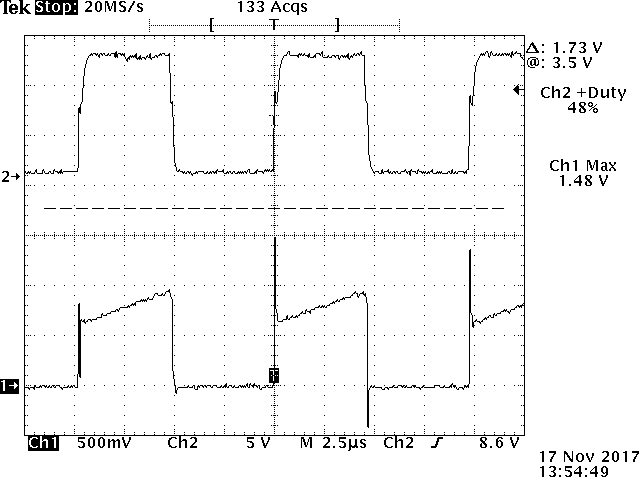
\includegraphics[max width=0.7\linewidth]{/tex/2iteration/billeder/Realisering/CS_U_filter.png}
	\caption{Oprindeligt current-sense signal før filter}
	\label{fig:CS_U_filter}
\end{figure}

\noindent Med den valgte stige tid på $100ns$, kan båndbredden af filteret estimeres:
\begin{equation} \label{filter_BW}
BW \approx \frac{0.34}{t_r} = \frac{0.34}{100ns} \approx 3.4M\hertz
\end{equation}

\noindent Kondensatoren fastholdes på $C_f=100pF$. Ud fra kondensatoren og den ønskede båndbredde i filteret, regnes modstanden.
\begin{equation} \label{filter_R}
R_f = \frac{1}{2 \cdot \pi \cdot BW \cdot C_f} = \frac{1}{2 \cdot \pi \cdot 3.4M\hertz \cdot 100pF} = 468.1\ohm
\end{equation}

\noindent Her vælges en modstand på $464\ohm$.




